
\chapter{Motivation for Topologists}

\chapterquote{%
I'm a goddess \emph{and} a nerd!}{%
Bright~\cite{Bri}}



\noindent
Higher-dimensional category theory \emph{can} be treated as a purely
algebraic subject, but that would be missing the point.  It is inherently
topological in nature: the diagrams that one naturally draws to illustrate
higher-dimensional structures can be taken quite literally as pieces of
topology.  Examples of this are the braidings in a braided%
%
\index{monoidal category!braided}
%
monoidal
category and the pentagon%
%
\index{pentagon}
%
appearing in the definitions of both monoidal
category and $A_\infty$-space.%
%
\index{A-@$A_\infty$-!space}
%

This section is an informal description of what higher-dimensional category
theory is and might be, and how it is relevant to topology.  Grothendieck,
for instance, suggested that tame topology should be the study of
$n$-groupoids;%
%
\index{n-groupoid@$n$-groupoid}
%
others have hoped that an $n$-category of cobordisms between cobordisms
between \ldots\ will provide a clean setting for topological quantum field
theory; and there is convincing evidence that the whole world of
$n$-categories is a mirror of the world of homotopy groups of spheres.

There are no real theorems, proofs, or definitions here.  But to whet your
appetite, here is a question to which we will reach an answer by the end:

\paragraph*{Question} What is the close connection between the following two
facts? 
%
\begin{description}
\item[A] No-one ever got into trouble for leaving out the brackets in a
tensor product of several objects (abelian groups, etc.).  For instance, it
is safe to write $A\otimes B\otimes C$ instead of $(A\otimes B)\otimes C$
or $A\otimes (B\otimes C)$.%
%
\index{associativity}
%

\item[B] There exist non-trivial knots%
%
\index{knot}
%
in $\reals^3$.
\end{description}


\section*{The very rough idea}
\ucontents{section}{The very rough idea}
%
%
\index{arrow|(}
%

In ordinary category theory we have diagrams of objects and arrows such as
\[
\gfstsu\ \gonesu\ \gzersu\ \gonesu\ \gzersu\ \gonesu\ \glstsu\ .
\]
We can imagine more complex category-like structures in which there
are diagrams such as
\[
\epsfig{file=higher.eps}.
\]
This looks like an electronic circuit diagram or a flow chart; the unifying
idea is that of `information flow'. It can be redrawn as
\[
\epsfig{file=plumbing.eps,height=62mm},
\]
which looks like a surface or a diagram from topological quantum field
theory.%
%
\index{topological quantum field theory}
%

We can also use diagrams like this to express algebraic laws such as
commutativity:
%
\begin{center}
\setlength{\unitlength}{1mm}
\begin{picture}(55,27)(0,3)
% main article
\cell{5}{6}{bl}{\epsfig{file=comm.eps}}
% LHS
\cell{5.5}{29.2}{r}{x}
\cell{15}{29}{l}{y}
\cell{5.5}{22}{r}{y}
\cell{15}{22.2}{l}{x}
\cell{10}{5}{t}{y\cdot x}
% RHS
\cell{40.5}{29.2}{r}{x}
\cell{50}{29}{l}{y}
\cell{45}{5}{t}{x\cdot y}
\end{picture}
.
\end{center}
%
The fact that two-dimensional TQFTs%
%
\index{topological quantum field theory}
%
are the same as commutative Frobenius%
%
\index{Frobenius algebra}%
%
\index{algebra!Frobenius}
%
algebras is an example of an explicit link between the spatial and
algebraic aspects of diagrams like these.

Moreover, if we allow crossings, as in the commutativity diagram or as in
\[
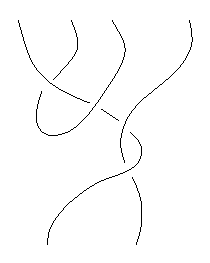
\epsfig{file=braid.eps,height=25mm,width=50mm},
\]
then we obtain pictures looking like knots; and as we shall see, there are
indeed relations between knot theory and higher categorical structures.

So the idea is:
%
\begin{trivlist} \item
\fbox{\parbox{0.98\textwidth}{\centering%
Ordinary category theory uses $1$-dimensional arrows $\go$\\
Higher-dimensional category theory uses higher-dimensional arrows}}
\end{trivlist}
%
The natural topology of these higher-dimensional arrows is what makes
higher-dimensional category theory an inherently topological subject.%
%
\index{arrow|)}
%

We will be concerned with structures such as operads, generalized operads
(of which the variety familiar to homotopy theorists is a basic special
case), multicategories, various flavours of monoidal categories, and
$n$-categories; in this introduction I have chosen to concentrate on
$n$-categories.  Terminology: an $n$-category (or `higher-dimensional
category')%
%
\index{higher-dimensional category@`higher-dimensional category'}
%
is not a special kind of category, but a generalization of the
notion of category; compare the usage of `quantum group'.  A $1$-category%
%
\index{one-category@1-category}
%
is the same thing as an ordinary category, and a $0$-category%
%
\index{zero-category@0-category}
%
is just a
set.


\section*{$n$-categories}
\ucontents{section}{$n$-categories}

Here is a very informal

\paragraph*{`Definition'} Let $n\geq 0$.  An
\demph{$n$-category}%
%
\index{n-category@$n$-category!definitions of!informal}
%
consists of 
%
\begin{itemize}
\item \demph{0-cells}%
%
\index{cell!n-category@of $n$-category}
%
or \demph{objects}, $A, B, \ldots$
\item \demph{1-cells} or \demph{morphisms}, drawn as
$A \cone{f} B$ 
\item \demph{2-cells} $A \ctwomult{f}{g}{\alpha} B$ (`morphisms between
morphisms') 
\item \demph{3-cells}
$A \cthreecellmult{f}{g}{\alpha}{\beta}{\Gamma} B$ 
(where the arrow
labelled $\Gamma$ is meant to be going in a direction perpendicular to the
plane of the paper)
\item \ldots
\item all the way up to \demph{$n$-cells}
\item various kinds of \demph{composition}, e.g.
\[
\begin{array}{ccc}
A \cone{f} B \cone{g} C					&\textrm{gives}
&A \cone{g\of f} C 			\\
% &&\textrm{(as usual)}			\\
A \cthreemult{f}{g}{h}{\alpha}{\beta} B			&\textrm{gives}
&A \ctwomult{f}{h}{\beta\of\alpha} B	
\label{p:2-cell-comps}
\\
A \ctwomult{f}{g}{\alpha} A' \ctwomult{f'}{g'}{\alpha'}
A'' 							&\textrm{gives}
&A \ctwomult{f'\of f}{g'\of g}{\!\!\!\!\!\!\!\!\alpha' *\alpha} A'',
\end{array}
\]
and so on in higher dimensions; and similarly \demph{identities}.
\end{itemize}
%
These compositions are required to `all fit together nicely'---a phrase
hiding many subtleties. 
% 
\demph{$\omega$-categories}%
%
\index{omega-category@$\omega$-category!informal definition of}
%
(also known as \demph{$\infty$-categories}) are
defined similarly, by going on up the dimensions forever instead of stopping
at $n$.

\paragraph*{} There is nothing forcing us to make the cells spherical
here.  We could, for instance, consider cubical structures, in which
2-cells look like
%
\begin{diagram}[size=2em,abut]
\bullet	&\rTo		&\bullet\\
\dTo	&\Downarrow	&\dTo	\\
\bullet	&\rTo		&\bullet\makebox[0em]{.}	
\end{diagram}
%
This is an inhabitant of the `zoo of structures' mentioned earlier, but is
not an $n$-category as such.  (See~\ref{sec:cl-strict} and~\ref{sec:wk-dbl}
for more on this particular structure.)

\paragraph*{Critical Example} Any topological space $X$ gives rise to an
$\omega$-category $\Pi_\omega X$%
% 
\glo{fundomega}
%
(its \demph{fundamental $\omega$-groupoid}),%
%
\index{fundamental!omega-groupoid@$\omega$-groupoid}
%
 in which
%
\begin{itemize}
\item 0-cells are points of $X$, drawn as $\ \blob$
\item 1-cells are paths%
%
\index{path}
%
in $X$ (maps $[0,1] \go X$), drawn as
$\gfstsu\gonesu\glstsu$ ---though whether that is meant to be a picture in
the space $X$ or the $\omega$-category $\Pi_\omega X$ is deliberately
ambiguous; the idea is to blur the distinction between geometry and
algebra
\item 2-cells are homotopies of paths (relative to endpoints), drawn as
$\gfstsu\gtwomultsu\glstsu$
\item 3-cells are homotopies%
%
\index{homotopy!higher}
%
of homotopies of paths (that is, suitable maps
$[0,1]^3 \go X$)
\item \ldots
\item composition is by pasting paths and homotopies.
\end{itemize}
%
(The word `groupoid'%
%
\index{groupoid}
%
means that all cells of dimension higher than zero are
invertible.)

$\Pi_\omega X$ should contain all the information you want about $X$ if
your context is `tame topology'.  In particular, you should be able to
compute from it the homotopy, homology and cohomology of $X$.  You can also
truncate after $n$ steps in order to obtain $\Pi_n X$,%
% 
\glo{fundn}
%
the
\demph{fundamental $n$-groupoid} of $X$; for instance, $\Pi_1 X$ is the
familiar fundamental groupoid.

\paragraph{Alert}%
%
\index{n-category@$n$-category!weak vs. strict@weak \vs.\ strict|(}
%
As you may have noticed, composition in $\Pi_\omega X$
is not genuinely associative; nor is it unital, and nor are the cells
genuinely invertible%
%
\index{invertibility}
%
(only up to homotopy).  We are therefore interested in
\demph{weak} $n$-categories, where the `fitting together nicely' only
happens up to some kind of equivalence, rather than \demph{strict}
$n$-categories, where associativity and so on hold in the strict sense.

To define strict $n$-categories precisely turns out to be easy.  To define
weak $n$-categories,%
%
\index{n-category@$n$-category!definitions of}
%
we face the same kind of challenge as algebraic
topologists did in the 1960s, when they were trying to state the exact
sense in which a loop%
%
\index{loop space}
%
space is a topological group.%
%
\index{group!topological}
%
 It is clearly not a group in the literal sense, as composition of paths is
not associative; but it is associative up to homotopy, and if you pick
specific homotopies to do this job then these homotopies obey laws of their
own---or at least, obey them up to homotopy; and so on.  At least two
precise formulations of `group up to (higher) homotopy' became popular:
Stasheff's%
%
\index{Stasheff, Jim}
%
$A_\infty$-spaces%
%
\index{A-@$A_\infty$-!space}
%
and Segal's%
%
\index{Segal, Graeme}
%
special $\Delta$-spaces.%
%
\index{Delta-space@$\Delta$-space}%
%
\index{special}%
%
\index{simplicial space}
%
 (More exactly,
these are notions of monoid or semigroup up to homotopy; the inverses%
%
\index{invertibility}
%
are
dealt with separately.)

The situation for weak $n$-categories is similar but more extreme: there
are something like a dozen proposed definitions and, as mentioned in the
Introduction, not much has been proved about how they relate to one
another.  Happily, we can ignore all this here and work informally.  This
means that nothing in the rest of this section is true with any degree of
certainty or accuracy.

At this point you might be thinking: can't we do away with this difficult
theory of weak $n$-categories and just stick to the strict ones?  The
answer is: if you're interested in topology, no.  The difference between
the weak and strict theories is genuine and nontrivial: for while it is
true that every weak $2$-category is equivalent%
%
\index{coherence!n-categories@for $n$-categories}
%
to some strict one, and so
it is also true that homotopy $2$-types%
%
\index{homotopy!type}
%
can be modelled by strict
$2$-groupoids, neither of these things is true in dimensions $\geq 3$.  For
instance, there exist spaces $X$ (such as the 2-sphere%
%
\index{sphere}
%
$S^2$) for which the
weak $3$-category%
%
\index{fundamental!3-groupoid}
%
$\Pi_3 X$ is not equivalent%
%
\index{coherence!tricategories@for tricategories}
%
to any strict $3$-category.

For the rest of this section, `$n$-category' will mean `weak $n$-category'.
The strict ones are very much the lesser-spotted species.%
%
\index{n-category@$n$-category!weak vs. strict@weak \vs.\ strict|)}
%

\paragraph*{Some More Examples} of $\omega$-categories:
%
\begin{description}
%
\item[\Top]%
% 
\glo{Top}
%
This is very similar to the $\Pi_\omega$ example above.  \Top\
has:
\begin{itemize}
\item 0-cells: topological spaces
\item 1-cells: continuous maps
\item 2-cells $X \ctwomult{f}{g}{} Y$: homotopies
between $f$ and $g$
\item 3-cells: homotopies between homotopies (that is, suitable maps
$[0,1]^2 \times X \go Y$)
\item \ldots
\item composition as expected.
\end{itemize}

\item[\fcat{ChCx}]
This $\omega$-category has:
\begin{itemize}
\item 0-cells: chain complexes%
%
\index{chain complex!omega-category of complexes@$\omega$-category of complexes}
%
(of abelian groups, say)
\item 1-cells: chain maps
\item 2-cells: chain homotopies%
%
\index{chain homotopy}
%
\item 3-cells $A\cthreecellmult{f}{g}{\alpha}{\beta}{\Gamma}B$: homotopies
between homotopies,% 
% 
\lbl{p:ch-hty-hty}\index{homotopy!higher}
%
that is, maps $\Gamma: A \go B$ of degree $2$ such that
$d\Gamma - \Gamma d = \beta - \alpha$
\item \ldots
\item composition: more or less as expected, but some choices are involved.
For instance, if you try to write down the composite of two chain
homotopies $\gfstsu\gtwomultsu\gzersu\gtwomultsu\glstsu$ then you will find
that there are two equally reasonable ways of doing it: one `left-handed',%
%
\index{handedness}
%
one `right-handed'.  This is something like choosing the parametrization
when deciding how to compose two loops in a space (usual choice: do
everything at double speed).  Somehow the fact that there is no canonical
choice means that the resulting $\omega$-category is bound to be weak.
\end{itemize}
%
In a reasonable world there ought to be a weak $\omega$-functor
$\fcat{Chains}: \fcat{Top} \go \fcat{ChCx}$.

\item[Cobord]%
%
\index{cobordism|(}\index{manifold!corners@with corners|(}%
\index{topological quantum field theory|(}
%
This is an $\omega$-category of cobordisms.  
% 
\begin{itemize}
\item 0-cells: 0-manifolds, where `manifold' means `compact, smooth, oriented
manifold'.  A typical 0-cell is 
$\ \stackrel{\uparrow}{\blob}\ \ 
\stackrel{\downarrow}{\blob}\ \ 
\stackrel{\uparrow}{\blob}\ \ 
\stackrel{\uparrow}{\blob}\ $.%
%
\item 1-cells: 1-manifolds with corners, that is, cobordisms between
0-manifolds, such as
%
\begin{center}
\setlength{\unitlength}{1mm}
\begin{picture}(30,30)(0,-5)
\cell{0}{0}{bl}{\epsfig{file=onecobord.eps}}
\cell{0.5}{21.5}{b}{\scriptstyle{\downarrow}}
\cell{10.5}{21.5}{b}{\scriptstyle{\downarrow}}
\cell{20.5}{21.5}{b}{\scriptstyle{\uparrow}}
\cell{30.5}{21.5}{b}{\scriptstyle{\uparrow}}
\cell{6.5}{-0.5}{t}{\scriptstyle{\downarrow}}
\cell{24.5}{-0.5}{t}{\scriptstyle{\uparrow}}
\end{picture}
\end{center}
%
(this being a 1-cell from a 4-point 0-manifold to a 2-point 0-manifold).
Atiyah-Segal-style TQFT stops here and takes \emph{isomorphism classes} of
the 1-cells just described, to make a category.  We avoid this (unnatural?)
quotienting out and carry on up the dimensions.
\item 2-cells: 2-manifolds with corners, such as
\[
\begin{array}[c]{c}
\epsfig{file=pants.eps}	
\end{array}
\ \ \textrm{or}\ \ 	
\begin{array}[c]{c}
\epsfig{file=twocobord.eps}	
\end{array}
\]
(leaving all the orientations off).  The right-hand diagram shows a 2-cell
$L \ctwomult{M}{M'}{N} L'$, where 
\[
L = \ \blob\ \ \blob\ ,
\diagspace 
L'=\ \blob\ \ \blob\ \ \blob\ \ \blob\ , 
\diagspace
M=\begin{array}[c]{c}
\epsfig{file=hoops.eps}
\end{array},
\diagspace
M'=\begin{array}[c]{c}
\epsfig{file=lines.eps}
\end{array},  
\]
and $N$ is the disjoint union of the two 2-dimensional sheets.
Khovanov~\cite{KhoFVI}%
%
\index{Khovanov, Mikhail}
%
discusses TQFTs with corners in the language of
2-categories; his approach stops here and take isomorphism classes of the
2-cells just described, to make a 2-category.  Again, we do not quotient
out but keep going up the dimensions.
\item 3-cells, 4-cells, \ldots\ are defined similarly
\item composition is gluing of manifolds.
\end{itemize}
%
Some authors discuss `extended TQFTs' using the notion of $n$-vector
space.%
%
\index{n-vector space@$n$-vector space}
%
A $0$-vector space is a complex number, a $1$-vector space is an ordinary
complex vector space, and $n$-vector spaces for higher $n$ are something
more sophisticated.  See the Notes below for references.%
%
\index{cobordism|)}\index{manifold!corners@with corners|)}
\index{topological quantum field theory|)}
%
\end{description}



\section*{Stabilization}
\ucontents{section}{Stabilization}
%
%
\index{stabilization|(}\index{n-category@$n$-category!degenerate|(}
%

So far we have seen that topological structures provide various good examples
of $n$-categories, and that alone might be enough to convince you that
$n$-categories are interesting from a topological point of view.  But the
relationship between topology and higher-dimensional category theory is
actually much more intimate than that.  To see how, we analyse certain
types of degenerate $n$-categories.  It will seem at first as if this is a
purely formal exercise, but before long the intrinsic topology will begin
to shine through.

\paragraph*{Some Degeneracies}

\begin{itemize}

\item A category%
%
\index{category!degenerate}
%
\cat{C} with only one object is the same thing as a
monoid%
% 
\lbl{p:degen-cat-monoid}%
%
\index{monoid!degenerate category@as degenerate category}
%
(semigroup with unit) $M$.  For if the single object of \cat{C} is
called $\star$, say, then \cat{C} just consists of the set
$\Hom(\star,\star)$ together with a binary operation of
composition and a unit element $1$, obeying the usual axioms.  So we have:
\[
\begin{array}{rcl}
\textrm{morphism in }\cat{C}	&=	&\textrm{element of }M		\\
\of \textrm{ in } \cat{C}	&=	&\cdot \textrm{ in }M.
\end{array}
\ \ \ 
\begin{array}{c}
\setlength{\unitlength}{1em}
\begin{picture}(7.4,2.6)(-3.7,-0.2)
% Object
\cell{0}{0}{c}{\star}
% LHS
\qbezier(-0.5,0)(-2.5,0)(-2.5,1.3)
\qbezier(-2.5,1.3)(-2.5,2.4)(-1.2,2.4)
\qbezier(-1.2,2.4)(-0.4,2.2)(-0.2,0.5)
\put(-0.2,0.5){\vector(0,-1){0}}
\cell{-2.7}{1.4}{r}{x}
% RHS
\qbezier(0.5,0)(2.5,0)(2.5,1.3)
\qbezier(2.5,1.3)(2.5,2.4)(1.2,2.4)
\qbezier(1.2,2.4)(0.4,2.2)(0.2,0.5)
\put(0.5,0.0){\vector(-1,0){0}}
\cell{2.7}{1.4}{l}{y}
\end{picture}
% \epsfig{file=monoid.ps}
\end{array}
\]

\item A 2-category%
%
\index{two-category@2-category!degenerate}
%
\cat{C} with only one $0$-cell is the same thing as a
monoidal category \cat{M}.  (Private thought: if \cat{C} has only one
$0$-cell then there are only interesting things happening in the top two
dimensions, so it must be \emph{some} kind of one-dimensional structure.)
This works as follows:
%
\begin{eqnarray*}
1\textrm{-cell in }\cat{C}	&=	&\textrm{object of }\cat{M}	\\
2\textrm{-cell in }\cat{C}	&=	&\textrm{morphism of }\cat{M}	\\
\textrm{composition } \ \gzersu\gonesu\gzersu\gonesu\gzersu\  \textrm{ in }
\cat{C} 
&=	
&\otimes \textrm{ of objects in }\cat{M}				\\
\textrm{composition } \ \gzersu\gthreemultsu\gzersu\  \textrm{ in } \cat{C}
&=	
&\of \textrm{ of morphisms in }\cat{M}.				\\
\end{eqnarray*}

\item A monoidal category%
%
\index{monoidal category!degenerate}
%
\cat{C} with only one object is\ldots\ well, if
we forget the monoidal structure for a moment then, as we have just seen,
it is a monoid whose elements are the morphisms of \cat{C} and whose
multiplication is the composition in \cat{C}.  Now, the monoidal structure
on \cat{C} provides not only a tensor product for objects, but also a
tensor product for morphisms: so the set of morphisms of \cat{C} has a
second multiplication on it, $\otimes$.  So a one-object monoidal category
is a set $M$ equipped with two monoid structures that are in some sense
compatible (because of the axioms on a monoidal category).  A well-known
result~(\ref{lemma:EH})%
%
\index{Eckmann--Hilton argument}
%
says that in this situation, the two
multiplications are in fact equal and commutative.  So, a one-object
monoidal category is a commutative monoid.

This is, essentially, the argument often used to prove that the higher
homotopy groups are abelian, or that the fundamental group of a topological
group is abelian.  In fact, we can deduce that $\pi_2$%
%
\index{homotopy!group}
%
is abelian from our
`results' so far:

\textbf{Corollary:} $\pi_2(X,x_0)$ is abelian, for any space $X$ with
basepoint $x_0$. 

\textbf{Proof:} The 2-category $\Pi_2 X$%
%
\index{fundamental!2-groupoid}
%
has a sub-2-category whose only
0-cell is $x_0$, whose only 1-cell is the constant path at $x_0$, and whose
2-cells are all the possible ones from $\Pi_2 X$---that is, are the
homotopies from the constant path to itself, that is, are the elements of
$\pi_2(X,x_0)$.  This sub-2-category is a 2-category with only one 0-cell
and one 1-cell, that is, a monoidal category with only one object, that is,
a commutative monoid.

\item Next consider a 3-category%
%
\index{three-category@3-category!degenerate}
%
with only one 0-cell and one 1-cell.  We
have not looked at (weak) 3-categories in enough detail to work this out
properly, but it turns out that such a 3-category is the same thing as a
braided monoidal category.  By definition, a \demph{braided%
%
\index{monoidal category!braided}
%
monoidal
category} is a monoidal category equipped with a map (a \demph{braiding})
\[
A\otimes B \goby{\beta_{A,B}} B\otimes A
\]
for each pair $(A,B)$ of objects, satisfying axioms \emph{not} including
that
\[
(A\otimes B \goby{\beta_{A,B}} B\otimes A \goby{\beta_{B,A}} A\otimes B)
= 1.
\]
The canonical example of a braided monoidal category (in fact, the braided
monoidal category freely generated by a single object) is \fcat{Braid}.%
% 
\glo{Braid}
%
 This
has:
%
\begin{itemize}
\item objects: natural numbers $0, 1, \ldots$
\item morphisms: braids,%
%
\index{braid}
%
for instance
\[
\begin{array}[c]{c}
\epsfig{file=braidmorphism.eps}
\end{array}
\diagspace\diagspace\diagspace
\begin{diagram}[height=10mm]
4 \\ \dTo \\ 4 \\
\end{diagram}
\]
(taken up to homotopy); there are no morphisms $m \go n$ when $m \neq n$
\item tensor: placing side-by-side (which on objects means addition)
\item braiding: left over right, for instance
\[
\begin{array}[c]{c}
\epsfig{file=braiding.eps}
\end{array}
\diagspace\diagspace
\begin{diagram}[height=10mm]
3+2 \\ \dTo<{\beta_{3,2}} \\ 2+3 \\
\end{diagram}
\]
(Note that $\beta_{n,m} \of \beta_{m,n}$ is not the identity braid.)
\end{itemize}

\item We are rapidly getting out of our depth, but nevertheless: we have
already considered $n$-categories that are only interesting in the top two
dimensions for $n= 1$, $2$, and $3$.  These are categories, monoidal
categories, and braided monoidal categories respectively.  What next?  For
$r\geq 4$, an $r$-category with only one $i$-cell for each $i<r-1$ is,
people believe, the same as a symmetric%
%
\index{monoidal category!symmetric}
%
monoidal category (that is, a
braided monoidal category in which $\beta_{B,A} \of \beta_{A,B} = 1$ for
all $A,B$).  So the situation has stabilized\ldots\ and this is meant to
make you start thinking of stabilization phenomena in homotopy.
\end{itemize}

\paragraph*{The Big Picture}  Let us assemble this information on
degeneracies systematically.  Define an \demph{$m$-monoidal $n$-category}%
%
\index{monoidal n-category@monoidal $n$-category}%
\index{m-monoidal n-category@$m$-monoidal $n$-category}
%
to be an $(m+n)$-category with only one $i$-cell for each $i<m$.  (This is
certainly some kind of $n$-dimensional structure, as there are only
interesting cells in the top $(n+1)$ dimensions.)  Here is what $m$-monoidal
$n$-categories are for some low values of $m$ and $n$, laid out in the
so-called `periodic%
%
\index{periodic table}
%
table'.  Explanation follows.

\begin{center}
% \begin{trivlist} \item
% \hspace*{-10mm}
\setlength{\unitlength}{0.92mm}
% \setlength{\unitlength}{1.03mm}
\begin{picture}(131,88)(-4,-11)
\place{69}{76}{$n$}
\place{-1}{32}{$m$}
\put(2,66){\line(1,0){125}}
\put(10,0){\line(0,1){72}}
\place{6}{62}{$0$}
\place{6}{54}{$1$}
\place{6}{44}{$2$}
\place{6}{34}{$3$}
\place{6}{24}{$4$}
\place{6}{14}{$5$}
\place{6}{4}{$6$}
\place{24}{70}{$0$}
\place{24}{62}{set}
\place{24}{54}{monoid}
\place{24}{46}{commutative}
\place{24}{42}{monoid}
\place{24}{34}{\ditto}
\place{24}{24}{\ditto}
\place{24}{14}{\ditto}
\place{24}{4}{\ditto}
\place{54}{70}{$1$}
\place{54}{62}{category}
\place{54}{56}{monoidal}
\place{54}{52}{category}
\place{54}{46}{braided}
\place{54}{42}{mon cat}
\place{54}{36}{symmetric}
\place{54}{32}{mon cat}
\place{54}{24}{\ditto}
\place{54}{14}{\ditto}
\place{54}{4}{\ditto}
\place{84}{70}{$2$}
\place{84}{62}{2-category}
\place{84}{56}{monoidal}
\place{84}{52}{2-category}
\place{84}{46}{braided}
\place{84}{42}{mon 2-cat}
\place{84}{34}{rhubarb}
\place{84}{26}{symmetric}
\place{84}{22}{mon 2-cat}
\place{84}{14}{\ditto}
\place{84}{4}{\ditto}
\place{114}{70}{$3$}
\place{114}{62}{3-category}
\place{114}{56}{monoidal}
\place{114}{52}{3-category}
\place{114}{46}{braided}
\place{114}{42}{mon 3-cat}
\place{114}{34}{rhubarb}
\place{114}{24}{rhubarb}
\place{114}{16}{symmetric}
\place{114}{12}{mon 3-cat}
\place{114}{4}{\ditto}
\qbezier[10](24,54)(39,58)(54,62)
\qbezier[20](24,44)(54,53)(84,62)
\qbezier[30](24,34)(69,48)(114,62)
\qbezier[30](24,24)(69,39)(114,54)
\qbezier[30](24,14)(69,29)(114,44)
\qbezier[30](24,4)(69,19)(114,34)
\qbezier[20](54,4)(84,14)(114,24)
\qbezier[10](84,4)(99,9)(114,14)
%
\qbezier(28,-11)(35.5,-8.5)(43,-6)
\put(28,-11){\vector(-4,-1){0}}
\cell{45}{-9}{l}{\textrm{:\ \ \ take just the one-object structures}}
\label{p:periodic-table}
\end{picture}
% \end{trivlist}
\end{center}

In the first row ($m=0$), a $0$-monoidal $n$-category is simply an
$n$-category: it is not monoidal at all.

In the next row ($m=1$), a $1$-monoidal $n$-category is a monoidal%
%
\index{monoidal n-category@monoidal $n$-category}
%
$n$-category, in other words, an $n$-category equipped with a tensor
product that is associative and unital up to equivalence of a suitable
kind.  For instance, a $1$-monoidal $0$-category is a one-object category
(a monoid), and a $1$-monoidal $1$-category is a one-object $2$-category (a
monoidal category).  A monoidal $2$-category can be \emph{defined} as a
one-object 3-category, or can be defined directly as a 2-category with
tensor.

We see from these examples, or from the general definition of $m$-monoidal
$n$-category, that going in the direction $\swarrow$ means restricting to
the one-object structures.

Now look at the third row ($m=2$).  We have already seen that a degenerate
monoidal category is a commutative monoid and a doubly-degenerate
3-category is a braided monoidal category.  It is customary to keep writing
`braided monoidal $n$-category' all along the row, but you can regard this
as nothing more than name-calling.

Next consider the first \emph{column} ($n=0$).  A one-object braided%
%
\index{monoidal category!braided!degenerate}
%
monoidal category is going to be a commutative monoid together with a
little extra data (for the braiding) satisfying some axioms, but in fact
this is trivial and we do not get anything new: in some sense, `you can't
get better than a commutative monoid'.  This gives the entry for $m=3,
n=0$, and the same applies all the way down the rest of the column.

A similar story can be told for the second column ($n=1$).  We saw---or
rather, I claimed---that for $m\geq 3$, an $m$-monoidal $1$-category is
just a symmetric monoidal category.  So again the column stabilizes, and
again the point of stabilization is `the most symmetric thing possible'.

The same goes in subsequent columns.  The `rhubarbs' could be replaced by
more terminology---for instance, the first would become `sylleptic%
%
\index{monoidal category!sylleptic}
%
monoidal
2-category'---but the details are not important here.

The main point is that the table stabilizes for $m\geq n+2$---just like
$\pi_{m+n}(S^m)$.  So if you overlaid a table of the homotopy groups%
%
\index{homotopy!group!sphere@of sphere}
%
of
spheres onto the table above then they would stabilize at the same points.
There are arguments to see why this should be so (and I remind you that
this is all very informal and by no means completely understood).  Roughly,
the fact that the archetypal braided monoidal category \fcat{Braid} is not
symmetric comes down to the fact that you cannot usually translate two
1-dimensional affine subspaces of 3-dimensional space past each other, and
this is the same kind of dimensional calculation as you make when proving
that the homotopy groups of spheres stabilize.%
%
\index{stabilization|)}
%

\paragraph{Answer} to the initial question:

\begin{description}
\item[A] Every weak 2-category is equivalent%
%
\index{coherence!bicategories@for bicategories}
%
to a strict one.
In particular, every (weak) monoidal category is equivalent to a strict one.
So, for instance, we can pretend that the monoidal category of abelian groups
is strict, making $\otimes$ strictly associative.%
%
\index{associativity}
%

\item[B] \emph{Not} every weak 3-category is equivalent%
%
\index{coherence!tricategories@for tricategories}
%
to a strict one.
We can construct a counterexample from what we have just done (details
aside).  Facts:
%
\begin{itemize}
\item a weak 3-category with one $0$-cell and one $1$-cell is a braided%
%
\index{monoidal category!braided}
%
monoidal category
\item a strict 3-category with one $0$-cell and one $1$-cell is a strict
symmetric monoidal category
\item any braided monoidal category equivalent to a symmetric monoidal
category is itself symmetric.
\end{itemize}
%
It follows that any non-symmetric braided monoidal category is a weak
3-category not equivalent to a strict one.  The canonical example is
\fcat{Braid} itself, which is non-symmetric precisely because the overpass
$\begin{array}{c} 
\epsfig{file=overpass.eps}
\end{array}$
cannot be deformed to the underpass 
$\begin{array}{c}
\epsfig{file=underpass.eps}
\end{array}$
in $\reals^3$.
\end{description}%
%
\index{n-category@$n$-category!degenerate|)}
%




\begin{notes}

Much has been written on the various interfaces between topology and higher
category theory.  I will just mention a few texts that I happen to have
come across.

Grothendieck%
%
\index{Grothendieck, Alexander}
%
puts the case that tame topology is really the study of
$\omega$-groupoids%
%
\index{omega-groupoid@$\omega$-groupoid}
%
in his epic~\cite{GroPS} letter to Quillen.  A seminal paper of
 Shum~\cite{Shum}%
%
\index{Shum, Mei Chee}
%
establishes connections between higher
categorical structures and knot%
%
\index{knot}
%
theory; see also Yetter~\cite{Yet}.

Another introduction to higher categories from a topological viewpoint,
with many similar themes to this one, is the first half of
Baez~\cite{BzIN}.%
%
\index{Baez, John}
%

Specifically 2-categorical approaches to topological quantum field theory%
%
\index{topological quantum field theory}
%
can be found in Tillmann~\cite{Till}%
%
\index{Tillmann, Ulrike}
%
and Khovanov~\cite{KhoFVI}.%
%
\index{Khovanov, Mikhail}
%
$n$-vector spaces%
%
\index{n-vector space@$n$-vector space}
%
are explained in Kapranov%
%
\index{Kapranov, Mikhail}
%
and Voevodsky~\cite{KV},%
%
\index{Voevodsky, Vladimir}
%
and
their possible role in topological field theory is discussed in
Lawrence~\cite{Law}.%
%
\index{Lawrence, Ruth}
%

The periodic%
%
\index{periodic table}
%
table is an absolutely fundamental object of mathematics, only
discovered quite recently (Baez%
%
\index{Baez, John}
%
and Dolan~\cite{BDHDA0}),%
%
\index{Dolan, James}
%
although
foreshadowed in the work of Breen%
%
\index{Breen, Lawrence}
%
and of Street%
%
\index{Street, Ross}
%
and the Australian school.  That the table stabilizes for $m\geq n+2$ is
the `Stabilization%
%
\index{Stabilization Hypothesis}
%
Hypothesis'.  To state it precisely one needs to set up all the appropriate
definitions first.  A form of it has been proved by Simpson~\cite{SimOBB},%
%
\index{Simpson, Carlos}
%
and a heuristic argument in the semistrict case has been given by
Crans~\cite[3.8]{CraBSS}.%
%
\index{Crans, Sjoerd}
%

I have made one economy with the truth: a (weak) monoidal%
%
\index{monoidal category!degenerate}
%
category with
only one object is not exactly a commutative monoid,%
%
\index{Eckmann--Hilton argument}
%
but rather a
commutative monoid equipped with a distinguished invertible element; see
Leinster~\cite[1.6(vii)]{GECM} for the reason.

One interesting idea not mentioned above is a higher categorical approach
to non-abelian cohomology:%
%
\index{cohomology}%
%
\index{homology}
%
specifically, $n$th cohomology should have
coefficients in an $n$-category.  This is explained in
Street~\cite[Introduction]{StrAOS}.%
%
\index{Street, Ross}
%

A serious and, of course, highly recommended survey of the proposed
definitions of weak $n$-category,%
%
\index{n-category@$n$-category!definitions of}
%
including ten such definitions, is my
own~\cite{SDN}.

\end{notes}



